\section{Uninformed Orderflow's Value to the Protocol} \label{section:protocol-lpcapital-value}

How much value does uninformed orderflow create for the protocol? Here we put forward an opinionated approach based on the expected protocol revenues that would materialize in a world with a nonzero protocol fee.

\subsection{A Protocol Fee Based Approach}

    The simplest approach that we have for determining the value that uninformed orderflow creates for the protocol is to analyze, under various fee switch scenarios, how much revenue the protocol earns as a result of uninformed orderflow.


    Utilizing the sandwich-adjusted value of uninformed orderflow, we can calculate a lower bound for the value that would go to the protocol as
        $v_{proto}(x) = (1+m_{sandwich}) \cdot x \cdot \gamma \phi,$
    for an order of volume $x$ and a sandwich multiple $m_{sandwich}$. The sandwich multiple can be computed by analyzing historical sandwich attacks and setting it as 

    \begin{equation} \label{eq:m-sandwich}
        m_{sandwich} = \frac{\text{dollars of front-run and back-run volume}}{\text{(dollars of uninformed volume) - (dollars of front-run and back-run volume)}}.
    \end{equation}
    
    Computing the numerator and the right side of the denominator of equation \ref{eq:m-sandwich} is straightforward, but computing the left side of the denominator is less obvious. Even if we know an order's observed markout, it is impossible to determine if that order was informed. With that said, we can create a lower bound on $m_{sandwich}$ by creating an upper bound on the dollars of uninformed volume, which itself is tractable. See appendix \ref{appendix:idendify-uninformed} for further details on orderflow information bounds.

    For the USDC-ETH-0.05\% Uni V3 pool, we estimate the following value of $m_{sandwich}$:
    \begin{equation}
        m_{sandwich} = \frac{{\text{13.5872\% of all pool volume}}}{(\text{33.0827\% of all pool volume}) - (\text{13.5872\% of all pool volume})} = 0.6969.
    \end{equation}
    
    % As we demonstrated before, on average, each dollar of sandwich victim volume leads approximately \$7 of front-/back-run volume. The sandwich victim volume composes approximately 2\% of the total volume, the ``bun'' volume composes approximately 14\% of the total volume, and the uninformed volume is a total of approximately 30\% of the volume. Thus, we can estimate that each \$$x$ of uninformed volume will lead to the following amount of ``bun'' volume

    %     \begin{align*}
    %         v_{\text{buns}}(x) = \frac{14\%}{16\%} \cdot x.
    %     \end{align*}
        
    That is, each unit of uninformed volume will beget approximately 0.70 more units of uninformed volume due to sandwiching. Recall from section \ref{subsection:sandwich-value-to-lps}, this method of attributing front- and back-running volume to an order given only the order's size is not accurate for a single order, but is accurate when used across many sandwich orders.

    Once we compute the sandwich multiple, we can utilize many potential protocol fees alongside the sandwich multiple to find the value that the protocol would make in the case where there was a protocol fee. See figure \ref{fig:proto-value-per-dollar-many-sandwich-multiple} for a visual depiction.

    \begin{figure}
        \centering
        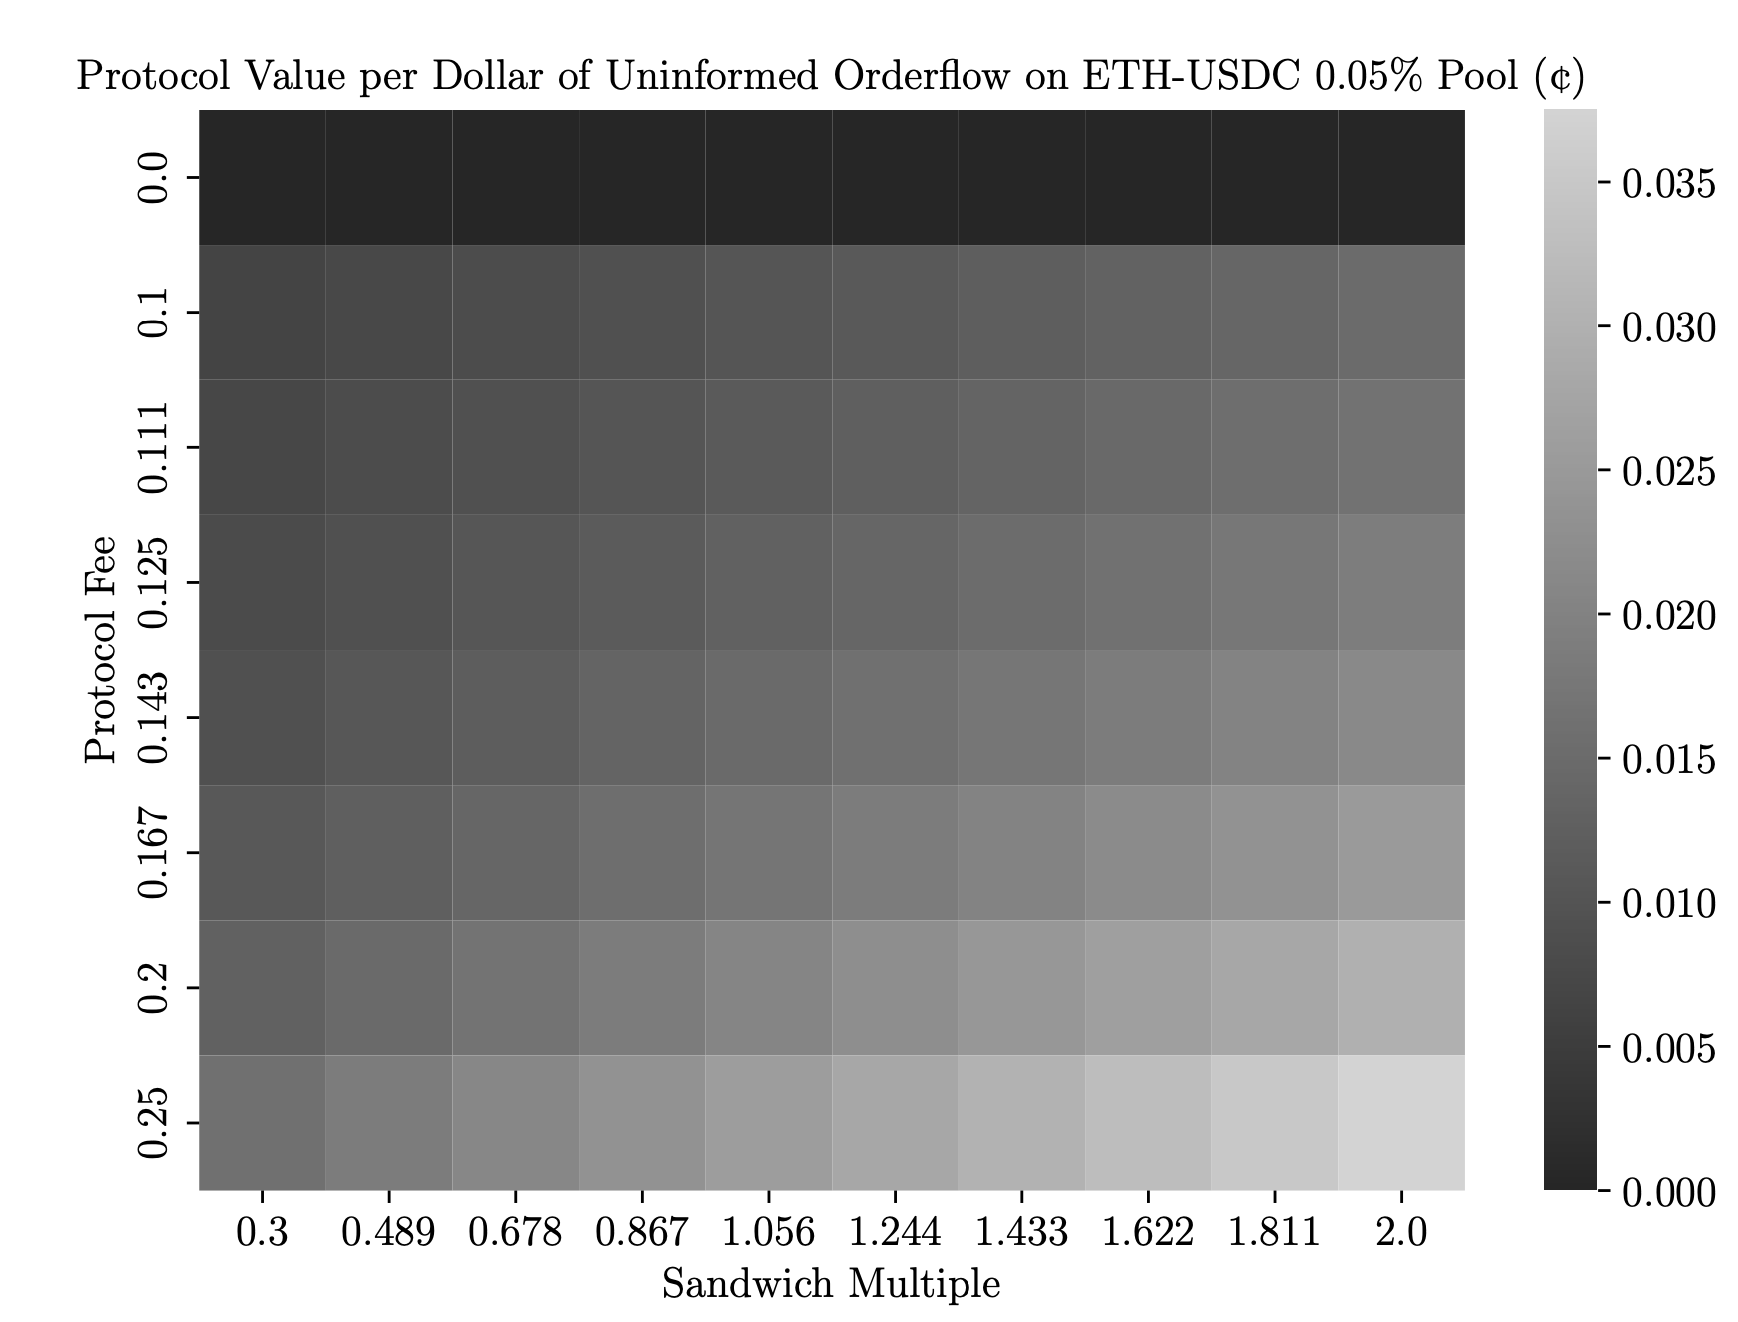
\includegraphics[scale=.33]{figs/protocol-value-per-orderflow-dollar.png}
        \caption{The value per dollar of uninformed orderflow for various protocol fees and sandwich multiples.}
        \label{fig:proto-value-per-dollar-many-sandwich-multiple}
    \end{figure}

    With current estimates of the sandwich multiple at $0.70$ on the USDC-ETH-0.05\% pool, the current value to the protocol is shown for each fee tier in figure \ref{fig:proto-value-per-dollar-current}.

    \begin{figure}[ht]
        \centering
        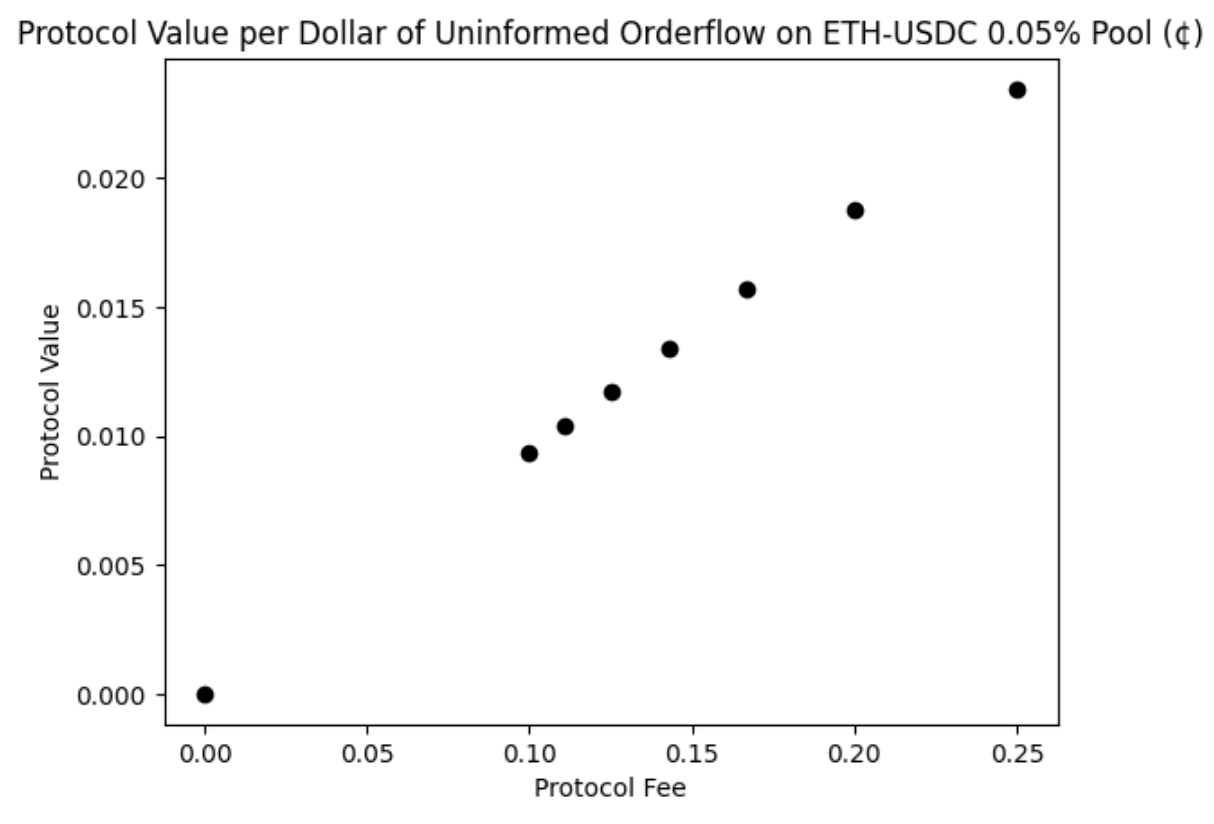
\includegraphics[scale=.33]{figs/protocol-value-vs-fee-current.png}
        \caption{The value per dollar of uninformed orderflow at the current empirically-observed sandwich multiple of 0.6969.}
        \label{fig:proto-value-per-dollar-current}
    \end{figure}

    It is important to note that these estimates are contingent on there being roughly the same amount of liquidity in a pool before and after a protocol fee is turned on. Due to the technical and political complexity of the protocol fee, we refrain from analysis of the impact that the protocol fee would have on liquidity. Nevertheless, it is intuitive that the amount of liquidity would decrease in pools that have higher protocol fees, and this would lead to smaller sandwich volumes. Our chart assumes that there is no relationship between the sandwich multiple and the protocol fee, which is not true.

    Thus, our dear reader now approaches a fork in the road. If one believes that small values of the protocol fee would not lead to a meaningful decrease in liquidity, then figure \ref{fig:proto-value-per-dollar-many-sandwich-multiple} demonstrates a lower bound on the average amount of protocol revenue generated from each dollar of uninformed orderflow. This would allow us to conclude our analysis with a simple description of the value of uninformed orderflow.

    On the other hand, if one believes that an implementation of the protocol fee would lead to a meaningful decrease in liquidity, then the orderflow values here would be over-approximations of the value that uninformed orderflow creates for the protocol. The next step in this line of research would be to model the relationship between the protocol fee and liquidity, then to model the relationship between the sandwich multiple and liquidity. While this is an excellent opportunity for future research, we do not model the relationship between a protocol fee and liquidity here.

    Aside from this approach ignoring the effect of the protocol fee on liquidity, it also possesses the obvious drawback that, at the time of writing, there is no protocol fee. This approach would thus lead us to the unfortunate result that uninformed orderflow currently has zero value for the protocol. In the following section, we formulate a number of alternative ways that the protocol could value orderflow.
    % describe why each of these other approaches are irredeemably insufficient ways of valuing uninformed orderflow.
    % Readers can decide, according to their own protocol fee political leanings, if this is too harsh of an underestimate of uninformed orderflow value to the protocol.

\subsection{Non-approaches}
    We now list a number of intuitive, yet, \textit{in our opinion}, flawed ways of valuing uninformed orderflow for the protocol. 
    % We specifically advise that the protocol not utilize the following methodologies for evaluating the value of uninformed orderflow.

    \textbf{Non-approach 1: Liquidity is inherently valuable}.

    Another approach to valuing orderflow is to see how much it would affect liquidity, then ascribe a value on liquidity itself. Accumulating more liquidity would put Uniswap in a position of strength relative to its competitors. For instance, increased Uniswap liquidity leads to an increased share of DEX aggregator volumes, which leads to decreased DEX aggregator volumes for Uniswap's DEX competitors. However, ascribing a number to the value this creates for the Uniswap protocol would be a perilous task, since even in a world where Uniswap defeats all competitors, the protocol must generate revenue in order for that market dominance value to accrete. Thus we would need to fall back to our previous protocol fee based approach.


    \textbf{Non-approach 2: Uniswap could generate revenue from other sources}.

    While it is also possible that the Uniswap protocol could generate revenue from other sources than the protocol fee, it would be inappropriate for us to speculate on the existence, let alone the size, of those revenue opportunities. The protocol may revisit this approach if there is a tangible proposal for generating protocol revenues in a way other than the protocol fee.


    \textbf{Non-approach 3: Uninformed orderflow increases the value of the token}.

    Yet another approach for quantifying the value that uninformed orderflow creates for the protocol would be to determine how much value uninformed orderflow would accrete to the token. While on its surface this approach resembles a value-based management approach to valuing uninformed orderflow, it is clear that uninformed orderflow itself will not create value for tokenholders unless there is a revenue source for the token. In order to utilize this method of valuing orderflow, we would either need to default back to our initial approach of assuming there is a protocol fee, or we would need to assume there is another source of revenue, which we refute in non-approach 2.

    A similar train of thought is to determine the relationship between uninformed orderflow and the price of the UNI token. An increase in UNI token value would allow us to grow the protocol's liquidity and volume. Still, this suffers from the issues raised in non-approach 1. %Yet, this begs the question of why UNI token holders would want to increase the usership of the protocol, considering the fact that usership itself does not accrete in revenue. 

    If one is instead optimizing not for the UNI token value, but for the UNI token value \textit{for current holders}, then this approach is more coherent, since increasing the UNI token value would allow current holders to sell the token and realize a gain. 
    % Unfortunately for these aspiring tokenholders, we will not entertain this use case as an approach that the protocol should use to value uninformed orderflow.

\subsection{Takeaways}
    We provide an approach to measuring the value that the protocol would receive from uninformed orderflow, assuming a future state where protocol fees are collected, and we find the amount of value that would be created for the protocol if a protocol fee were put in place. The main drawback to this approach is that we do not model the effect that an increase in protocol fee would have on pool liquidity.

    Although introducing the protocol fee requires us to make assumptions about future governance actions, we argue that this is the only coherent way of placing value on uninformed orderflow at this time. All other intuitive methods -- the inherent value of uninformed orderflow, Uniswap generating non-protocol fee revenue, and token price -- suffer from other issues that make them unsuitable as a method for valuing uninformed orderflow.